\subsection{Progettazione Architetturale}

\subsubsection{Divisione Oraria}
La seguente tabella rappresenta la distribuzione oraria dei ruoli per ogni componente del gruppo:
{
\rowcolors{2}{grigetto}{white}
\renewcommand{\arraystretch}{2}
\centering
\begin{longtable}[h!] { C{4cm} C{1cm} C{1cm} C{1cm} C{1cm} C{1cm} C{1cm} C{3cm}}
\caption{Tabella della divisione oraria della Progettazione Architetturale}\\
\rowcolor{darkblue}

\textcolor{white}{\textbf{Membro del gruppo}} & 
\textcolor{white}{\textbf{RE}} & 
\textcolor{white}{\textbf{AM}} & 
\textcolor{white}{\textbf{AN}} & 
\textcolor{white}{\textbf{PT}} & 
\textcolor{white}{\textbf{PR}} & 
\textcolor{white}{\textbf{VE}} & 
\textcolor{white}{\textbf{Ore complessive}}\\	
\endhead
        
\MC{}                     &  5 &  0 &  0 & 14 & 10 &  4 &  33 \\
\LD{}                     &  8 &  0 &  0 & 18 &  0 &  7 &  33 \\
\CE{}                     &  0 &  8 &  0 & 10 &  5 &  6 &  29 \\
\SE{}                     &  0 & 10 &  6 & 10 &  0 &  6 &  32 \\
\PF{}                     &  0 &  6 &  0 &  5 &  7 & 13 &  31 \\
\DF{}                     &  0 &  0 & 13 &  5 &  7 &  6 &  31 \\
\BR{}                     &  6 &  0 &  0 &  0 & 17 &  8 &  31 \\
\AT{}                     &  0 &  0 &  8 &  7 &  0 & 16 &  31 \\
\textbf{Ore totali ruolo} & 19 & 24 & 27 & 69 & 46 & 66 & 251 \\
		
\end{longtable}
}

La suddivisione delle ore svolte da ciascun componente del gruppo per ogni ruolo viene rappresentata nel seguente istogramma:
\begin{figure}[h]
	\centering
	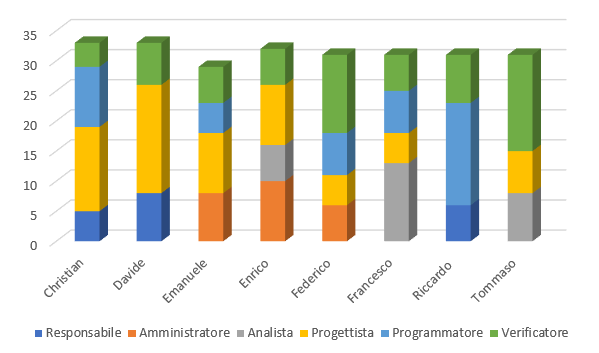
\includegraphics[scale=3]{Sezioni/Istogrammi/IstogrammaProgettArchitetturale.png}
	\caption{Disposizione ore per ruolo di ciascun componente della fase di Progettazione Architetturale}
\end{figure}

\clearpage

\subsubsection{Costo Risultante}
La seguente tabella rappresenta per ogni ruolo le ore totali investite e il corrispondente costo in euro:
{
\rowcolors{2}{grigetto}{white}
\renewcommand{\arraystretch}{2}
\centering
\begin{longtable}{ C{3cm} C{2cm} C{4cm}}
\caption{Tabella del costo risultante della Progettazione Architetturale}\\
\rowcolor{darkblue}

\textcolor{white}{\textbf{Ruolo}} & 
\textcolor{white}{\textbf{Totale ore}} & 
\textcolor{white}{\textbf{Costo ruolo in euro}}\\	
\endhead
        
Responsabile    &  19 &  570 \\
Amministratore  &  24 &  480 \\
Analista        &  27 &  675 \\
Progettista     &  69 & 1518 \\
Programmatore   &  46 &  690 \\
Verificatore    &  66 &  990 \\
\textbf{Totale} & 251 & 4923 \\	
        	
\end{longtable}
}

LaLa quantità di ore totali per ciascun ruolo viene rappresentata nel seguente areogramma:
\begin{figure}[h]
	\centering
	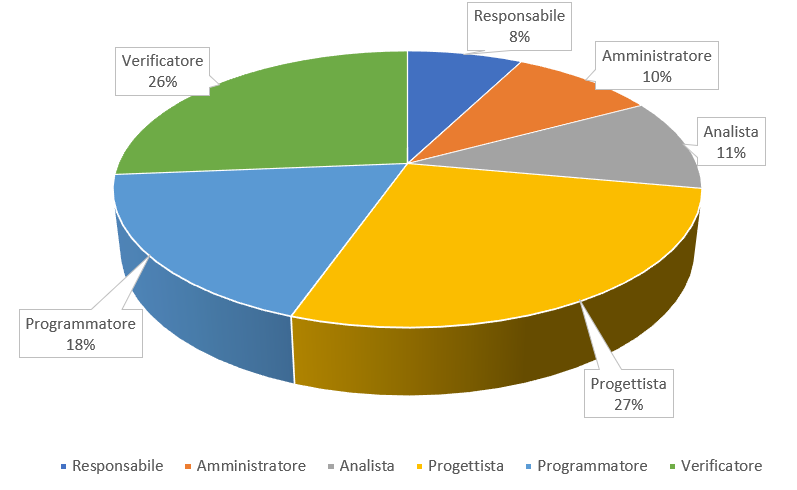
\includegraphics[scale=2.5]{Sezioni/Aerogrammi/AerogrammaProgettArchitetturale.png}
	\caption{Suddivisione ore per ruolo della fase di Progettazione Architetturale}
\end{figure}